\documentclass{article}
\usepackage{mathtools}
\usepackage[top=2in, bottom=1.5in, left=1in, right=1in]{geometry}
\usepackage{graphicx}
\usepackage[normalem]{ulem}
\usepackage{fancyhdr}
\usepackage{enumerate}
\pagestyle{fancyplain}

\lhead{PHYS 152 Section 10}

\rhead{A. Shawn Bandy 
(003635396)}

\begin{document}
\title{Lab \#3:  Oscilloscope and Function Generator}
\author{A. Shawn Bandy}
\date{February 18, 2013}
\maketitle
\begin{abstract}
This report presents our introduction to the oscilloscope and function generator.  According to our lab manual an oscilloscope "is a high-speed voltmeter that is used to display and measure rapid variations in potential differences."  The function generator is capable of sending out "time varying voltage."  We also used an {\it unknown function generator} - a DVD player and amplifier(?) with a CD with recordings of three signals.  We connected the function generators to the oscilloscope, took measurements and compared these measurements to settings on the generators.
\end{abstract}
\section{Data and Data Tables}
\begin{description}
\item[DATA SHEET \#1] \hfill
\begin{description}
\item[1. From procedure, part C.] \hfill \\
Amplitude value for square wave from DMM = 8.96 \\
Frequency value for square wave from function generator = 1.789 kHz 
\item[2. Square wave one: from part E, measurement using oscilloscope] \hfill \\
Peak-to-peak: \# of Divisions (vertical, to nearest 10\textsuperscript{th} of a division) = 3.7 \\
VOLTS/DIV setting = 5 \\
Amplitude of square wave = (0.5 * peak-to-peak voltage) = 9.85 V \\
Frequency from Oscilloscope: \\
\# of divisions (horizontal to nearest 10th) = 5.7 \\
SEC/DIV setting = 0.1 ms \\
Period of square wave calculated from above measurements = 0.00057  seconds\\
Frequency (calculated from period) = 1.754.4 kHz\\
\% difference in frequency value  = 0.019396
\item[3. Square wave two: from part G, measurement on oscilloscope] \hfill \\
Amplitude value of square wave from DMM = 2.0093 V \\
Frequency value for square wave from function generator = 8.99 kHz \\
Peak-to-peak: \# of Divisions (vertical, to the nearest 10\textsuperscript{th} of a division = 4.3 \\
VOLTS/DIV setting = 1
Amplitude of square wave = (0.5 * peak-to-peak voltage) = 2.15V \\
Frequency from Oscilloscope: \# of Divisions (horizontal to the nearest \textsuperscript{th} = 5.6 \\
SEC/DIV setting = 20 $\mu s$ \\
Period of square wave (calculated) = 8.929 kHz \\
\% difference in frequency value  = 0.006832 
\item[4. Which signal generator are you using?] {\it{Unknown Signal Generator}}
\end{description}
\item[DATA SHEEET \#2] \hfill
\begin{samepage}
{\small{
\begin{center}
	\begin{tabular}{| l | l | l | l | l | l | l | l |}
		\hline
		Signal \# &  \# of DIV & Volts per DIV & Volts & DIV per period & SEC/DIV & Period & Frequency (Hz)\\ \hline
		6 & 6 & 2 & 6 & 4.9 & .5 ms & 0.00245 & 408.163 \\ \hline
		8 & 4.2 & 5 & 10.5 & 5.1 & 1 ms & 0.0051 & 196.078 \\ \hline
		14 & 7.1 & 0.5  & 1.775 & 5.0 & 0.2 ms & 0.01 & 100 \\
		\hline
	\end{tabular}
\end{center}
}}
\end{samepage}
\end{description}
\section{Graphs}
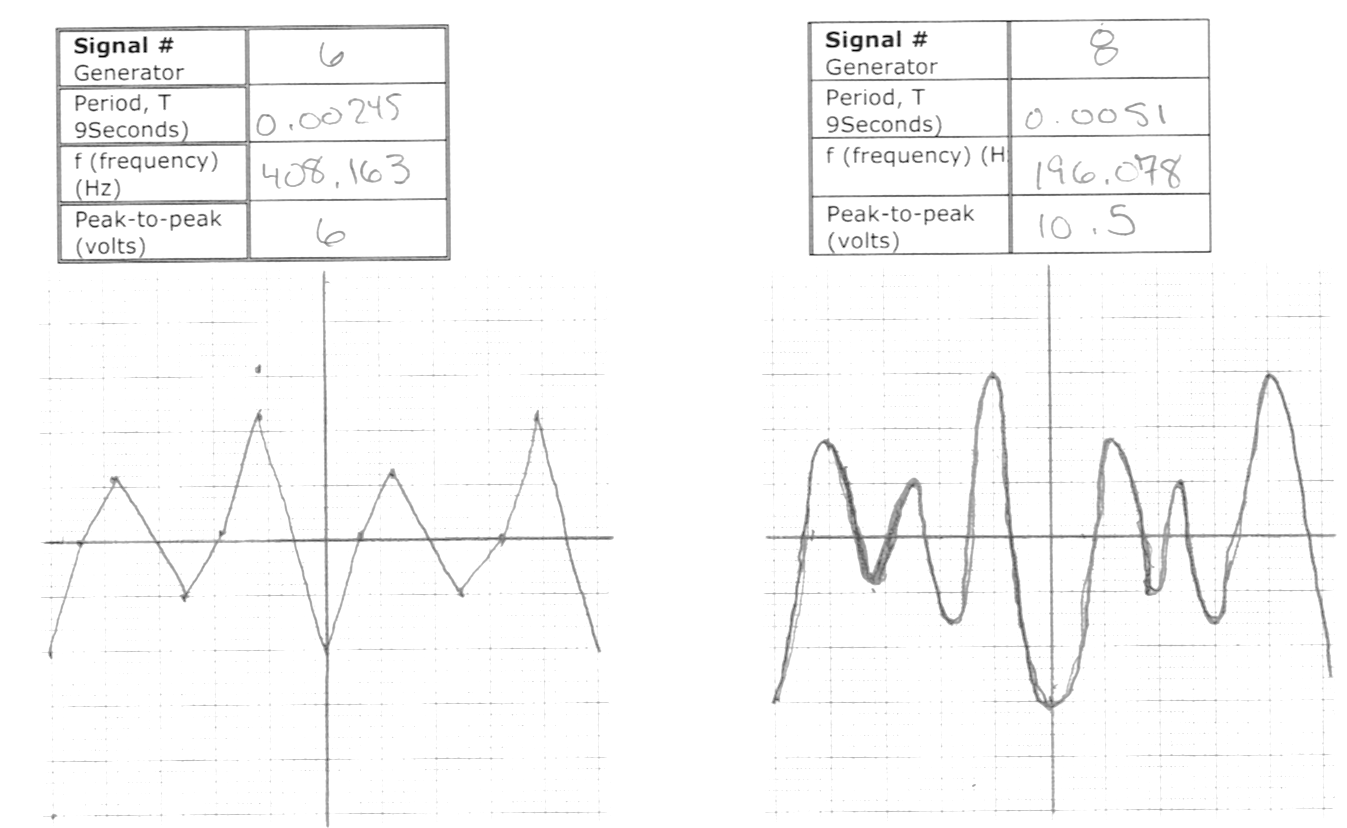
\includegraphics{graphs1_crop}
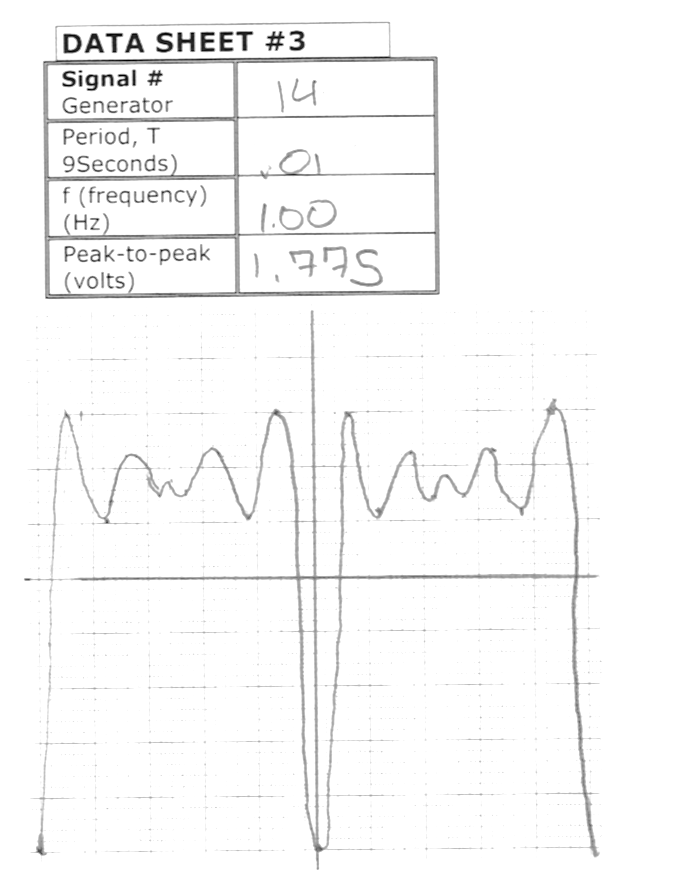
\includegraphics{graphs2_crop}
\section{Results}\hfill\\
For "square wave one", the percent difference in frequency value from function generator compared to frequency measurement from oscilloscope was \%1.9396.\\ \\
For "square wave two", the percent difference in frequency value from function generator compared to frequency measurement from oscilloscope was \%0.6832.\\
\section{Discussion}\hfill\\
\begin{samepage}
	We set the function generator to 9 volts and 1.8 kHz while it was connected to the digital multi-meter (DMM) to verify the output. We set the oscilloscope to 5 volts per division, 1 millisecond per division and set "Coupling" to "AC."  Once we had a stable display of the square wave on the oscilloscope, we took measurements by reading the vertical and horizontal marks.  Our measurements were limited to about 1 millimeter.  \\
	We reset the function generator to  2 volts and 9 kHz and adjusted to the oscilloscope so that the vertical and horizontal was maximally filled with one period of the wave without going beyond the boundaries of the display.  \\
	Finally we disconnected the function generator and connected the DVD/amplifier apparatus to the oscilloscope.  We took similar measurements of signals being generated by playing tracks 6, 8, and 14. \\
\end{samepage}
\section{Answers to Questions}
\begin{enumerate}[I]
\begin{samepage}
\item {\it There are controls on the function generator and the oscilloscope that have similar effects on the vertical size of the image.  Explain in your own words how adjustments on the two instruments are doing different things to change the vertical size of the signal on the oscilloscope screen.} \\ \\
The function generator can change the vertical size by increasing or decreasing the voltage of the signal while the oscilloscope only changes the vertical scale.  The oscilloscope, in other words, does not alter the signal just how it is displayed.\\
\end{samepage}
\begin{samepage}
\item {\it Answer the same questions as in I about the two instruments, but this time regarding controls that affect the horizontal size of the image on the screen.}\\ \\
The function generator can alter the frequency of the signal which is the horizontal axis of the oscilloscope display.  The oscilloscope can scale the period but it does not alter the signal itself.\\
\end{samepage}
\begin{samepage}
\item {\it One aspect of the image on the oscilloscope screen can be controlled only by the function generator.  What is that aspect, and why can't the oscilloscope change it?}\\ \\
The function generator can change the function - the "shape" of the function as it appears on the oscilloscope. \\
\end{samepage}
\end{enumerate}
\end{document}